\documentclass[border=10pt]{standalone}
\usepackage{tikz}
\usetikzlibrary{shapes.geometric, shapes.symbols, arrows.meta, positioning, calc, shadows}

\begin{document}
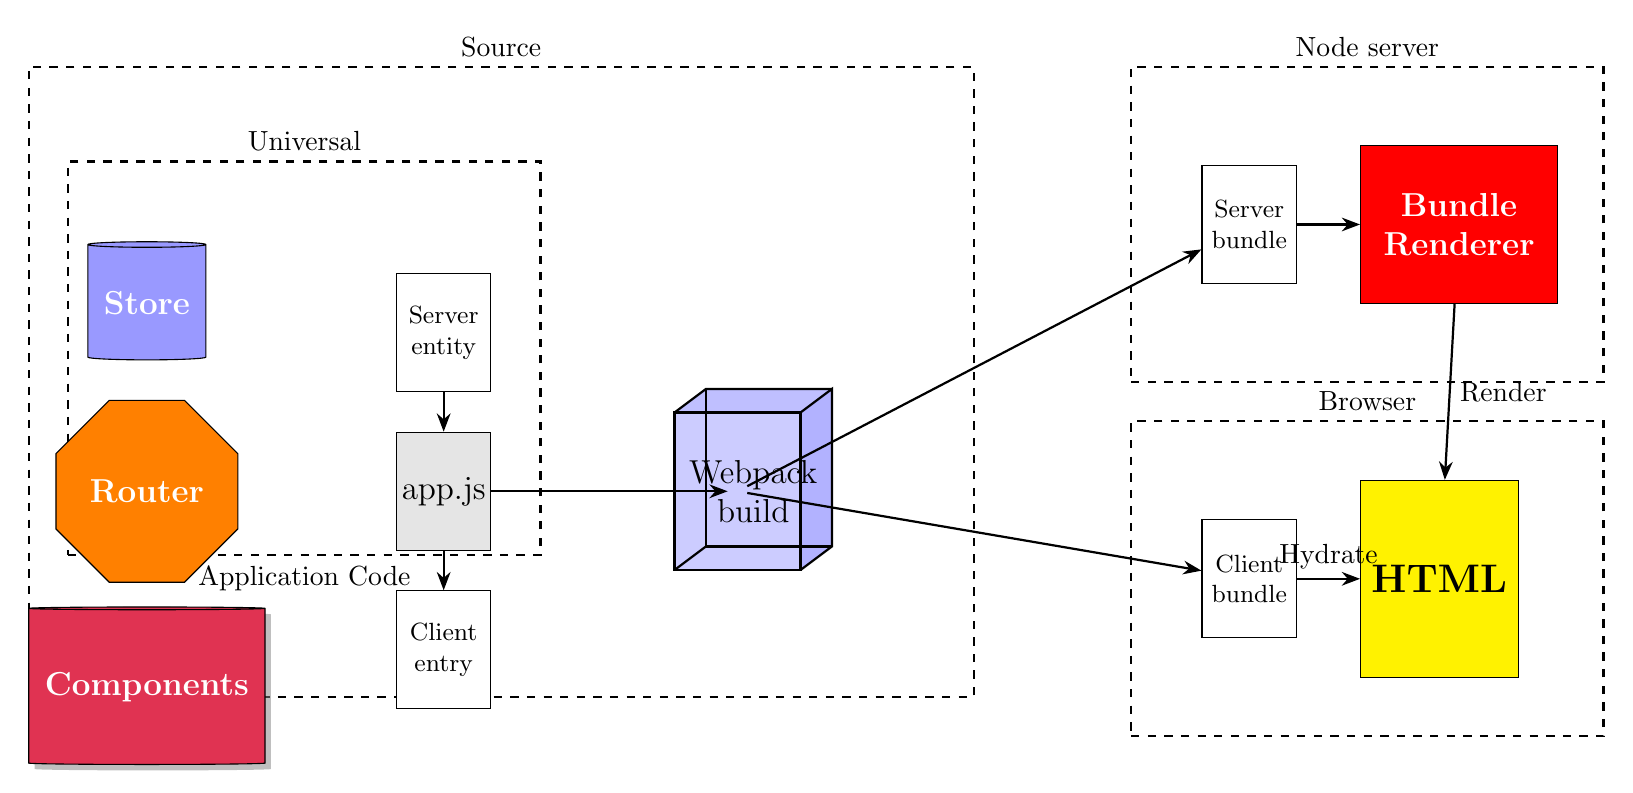
\begin{tikzpicture}[
    node distance=1cm,
    >=Stealth,
    doc/.style={rectangle, draw, minimum width=1.2cm, minimum height=1.5cm, 
                append after command={
                    ([xshift=-2mm, yshift=-2mm]\tikzlastnode.north east) -- 
                    (\tikzlastnode.north east) -- 
                    ([xshift=-2mm, yshift=-2mm]\tikzlastnode.north east) -- cycle
                }},
    container/.style={draw, dashed, thick, inner sep=8mm},
    ]

    % Source container
    \node[container, minimum width=12cm, minimum height=8cm, label={[anchor=south]north:Source}] (source) at (0,0) {};
    
    % Universal Application Code container
    \node[container, minimum width=6cm, minimum height=5cm, label={[anchor=south]north:Universal}, label={[anchor=north]south:Application Code}] (uac) at (-2.5,0.3) {};
    
    % Store
    \node[cylinder, draw, fill=blue!40, minimum height=1.5cm, minimum width=1.5cm, 
          shape aspect=0.3, shape border rotate=90] (store) at (-4.5, 1) {};
    \node[white, font=\large\bfseries] at (store) {Store};
    
    % Router
    \node[regular polygon, regular polygon sides=8, draw, fill=orange, 
          minimum size=2.5cm, below=0.5cm of store] (router) {};
    \node[white, font=\large\bfseries] at (router) {Router};
    
    % Components
    \node[cylinder, draw, fill=purple!60!red!80, minimum height=2cm, minimum width=3cm,
          shape aspect=0.15, shape border rotate=90, drop shadow,
          below=0.3cm of router] (components) {};
    \node[white, font=\large\bfseries] at (components) {Components};
    
    % app.js
    \node[doc, fill=black!10, right=2cm of router] (appjs) {};
    \node[font=\large] at (appjs) {app.js};
    
    % Server entity
    \node[doc, fill=white, above=0.5cm of appjs] (server_entity) {};
    \node[font=\small, align=center] at (server_entity) {Server\\entity};
    
    % Client entry
    \node[doc, fill=white, below=0.5cm of appjs] (client_entry) {};
    \node[font=\small, align=center] at (client_entry) {Client\\entry};
    
    % Webpack build
    \node[right=3cm of appjs] (webpack_center) {};
    \begin{scope}[shift={(webpack_center)}]
        % 3D box for webpack
        \coordinate (A) at (-0.8,-1);
        \coordinate (B) at (0.8,-1);
        \coordinate (C) at (0.8,1);
        \coordinate (D) at (-0.8,1);
        \coordinate (E) at (-0.4,-0.7);
        \coordinate (F) at (1.2,-0.7);
        \coordinate (G) at (1.2,1.3);
        \coordinate (H) at (-0.4,1.3);
        
        \fill[blue!20] (A) -- (B) -- (C) -- (D) -- cycle;
        \fill[blue!30] (B) -- (F) -- (G) -- (C) -- cycle;
        \fill[blue!25] (D) -- (C) -- (G) -- (H) -- cycle;
        \draw[thick] (A) -- (B) -- (C) -- (D) -- cycle;
        \draw[thick] (B) -- (F) -- (G) -- (C);
        \draw[thick] (D) -- (H) -- (G);
        \draw[thick] (E) -- (F);
        \draw[thick] (E) -- (H);
        \draw[thick] (E) -- (A);
        
        \node[font=\large, align=center] at (0.2,0) {Webpack\\build};
    \end{scope}
    
    % Arrows in source
    \draw[->, thick] (server_entity) -- (appjs);
    \draw[->, thick] (appjs) -- (client_entry);
    \draw[->, thick] (appjs) -- (webpack_center);
    
    % Node server container
    \node[container, minimum width=6cm, minimum height=4cm, 
          label={[anchor=south]north:Node server}] (node_server) at (11, 2) {};
    
    % Server bundle
    \node[doc, fill=white] (server_bundle) at (9.5, 2) {};
    \node[font=\small, align=center] at (server_bundle) {Server\\bundle};
    
    % Bundle Renderer
    \node[rectangle, draw, fill=red, minimum width=2.5cm, minimum height=2cm,
          right=0.8cm of server_bundle] (bundle_renderer) {};
    \node[white, font=\large\bfseries, align=center] at (bundle_renderer) {Bundle\\Renderer};
    
    % Browser container
    \node[container, minimum width=6cm, minimum height=4cm,
          label={[anchor=south]north:Browser}] (browser) at (11, -2.5) {};
    
    % Client bundle
    \node[doc, fill=white] (client_bundle) at (9.5, -2.5) {};
    \node[font=\small, align=center] at (client_bundle) {Client\\bundle};
    
    % HTML
    \node[doc, fill=yellow, minimum width=2cm, minimum height=2.5cm,
          right=0.8cm of client_bundle] (html) {};
    \node[font=\Large\bfseries] at (html) {HTML};
    
    % Arrows between sections
    \draw[->, thick] (webpack_center) -- (server_bundle);
    \draw[->, thick] (webpack_center) -- (client_bundle);
    \draw[->, thick] (server_bundle) -- (bundle_renderer);
    \draw[->, thick] (bundle_renderer) -- node[right] {Render} (html);
    \draw[->, thick] (client_bundle) -- node[above] {Hydrate} (html);
    
\end{tikzpicture}
\end{document}